\documentclass[handout]{beamer}
\usetheme{Berkeley}
\usecolortheme{whale}
\usepackage[english]{babel}
\usepackage{graphicx, amsmath, amsfonts, amsthm, mathtools, color, rotating, subfigure, setspace, enumerate, hyperref, floatrow}
\newfloatcommand{capbtabbox}{table}[][\FBwidth]

\title{Predicting Incidence of West Nile Virus}
\subtitle{Biostatistics M.S. Oral Exam}
\author{Christopher Aden}
\date{\today}

\begin{document}

\begin{frame}
\titlepage
\end{frame}

\section{Introduction}
\begin{frame}
\frametitle{Introduction}

\begin{description}
  \item[West Nile Virus (WNv):]\
    \begin{itemize}
      \item Transmitted by infected mosquitoes
      \item Symptoms: Fever, aching, fatigue, vomiting. Rarely: meningitis, encephalitis, death
      \item Occurs most frequently during peak mosquito seasons (late Spring--early Fall)
    \end{itemize}
  \item[Chicago's West Nile Virus Problem:]\
    \begin{itemize}
      \item Experienced first case in 2002.
      \item Established surveillance and management programs to control outbreaks.
	  \item Started monitoring/controlling mosquito populations in 2004.
    \end{itemize}
\end{description}
\end{frame}

\begin{frame}
\frametitle{The Data}
\begin{description}
\item[Surveillance Data (Traps)] \
\begin{itemize}
\item Data from geo-tagged mosquito traps.
\item Presence of WNv, species and counts.
\item Location: Latitude-Longitude, Street, Block
\item Time: Day, Month, Year
\end{itemize}
\item[Management Data (Sprays)]\
\begin{itemize}
\item Time (D-M-Y) and Location (Lat-Lon) of all insecticide sprays.
\end{itemize}
\item[NOAA Atmospheric and Weather Data (Weather)]\
\begin{itemize}
\item Collected at Chicago's two airports.
\item Time (D-M-Y)
\item Temperature (Max, Min, Avg), Atmospheric Pressure
\item Precipitation, Dew Point, Wind Speed, etc
\end{itemize}
\end{description}
\end{frame}

\begin{frame}
\frametitle{Main Questions}
    \begin{itemize}
	\item Controlling for location effects, is spraying an effective method of reducing the incidence of West Nile virus?
	\item What weather conditions influence WNv incidence and how?
	\item Can we develop a tool that has high sensitivity to detect West Nile virus, while still maintaining specificity?
    \end{itemize}
\end{frame}

\section{Inference, EDA}
\begin{frame}
\frametitle{Effect of Mosquito Species on WNv Incidence}
\begin{figure}[H]
\caption{1: \emph{C. Erraticus}, 2: \emph{C. Pipiens}, 3: \emph{C. Pipiens} or \emph{C. Restuans}, 4: \emph{C. Restuans}, 5: \emph{C. Salinarius}, 6: \emph{C. Tarsal}, 7: \emph{C. Territans}}
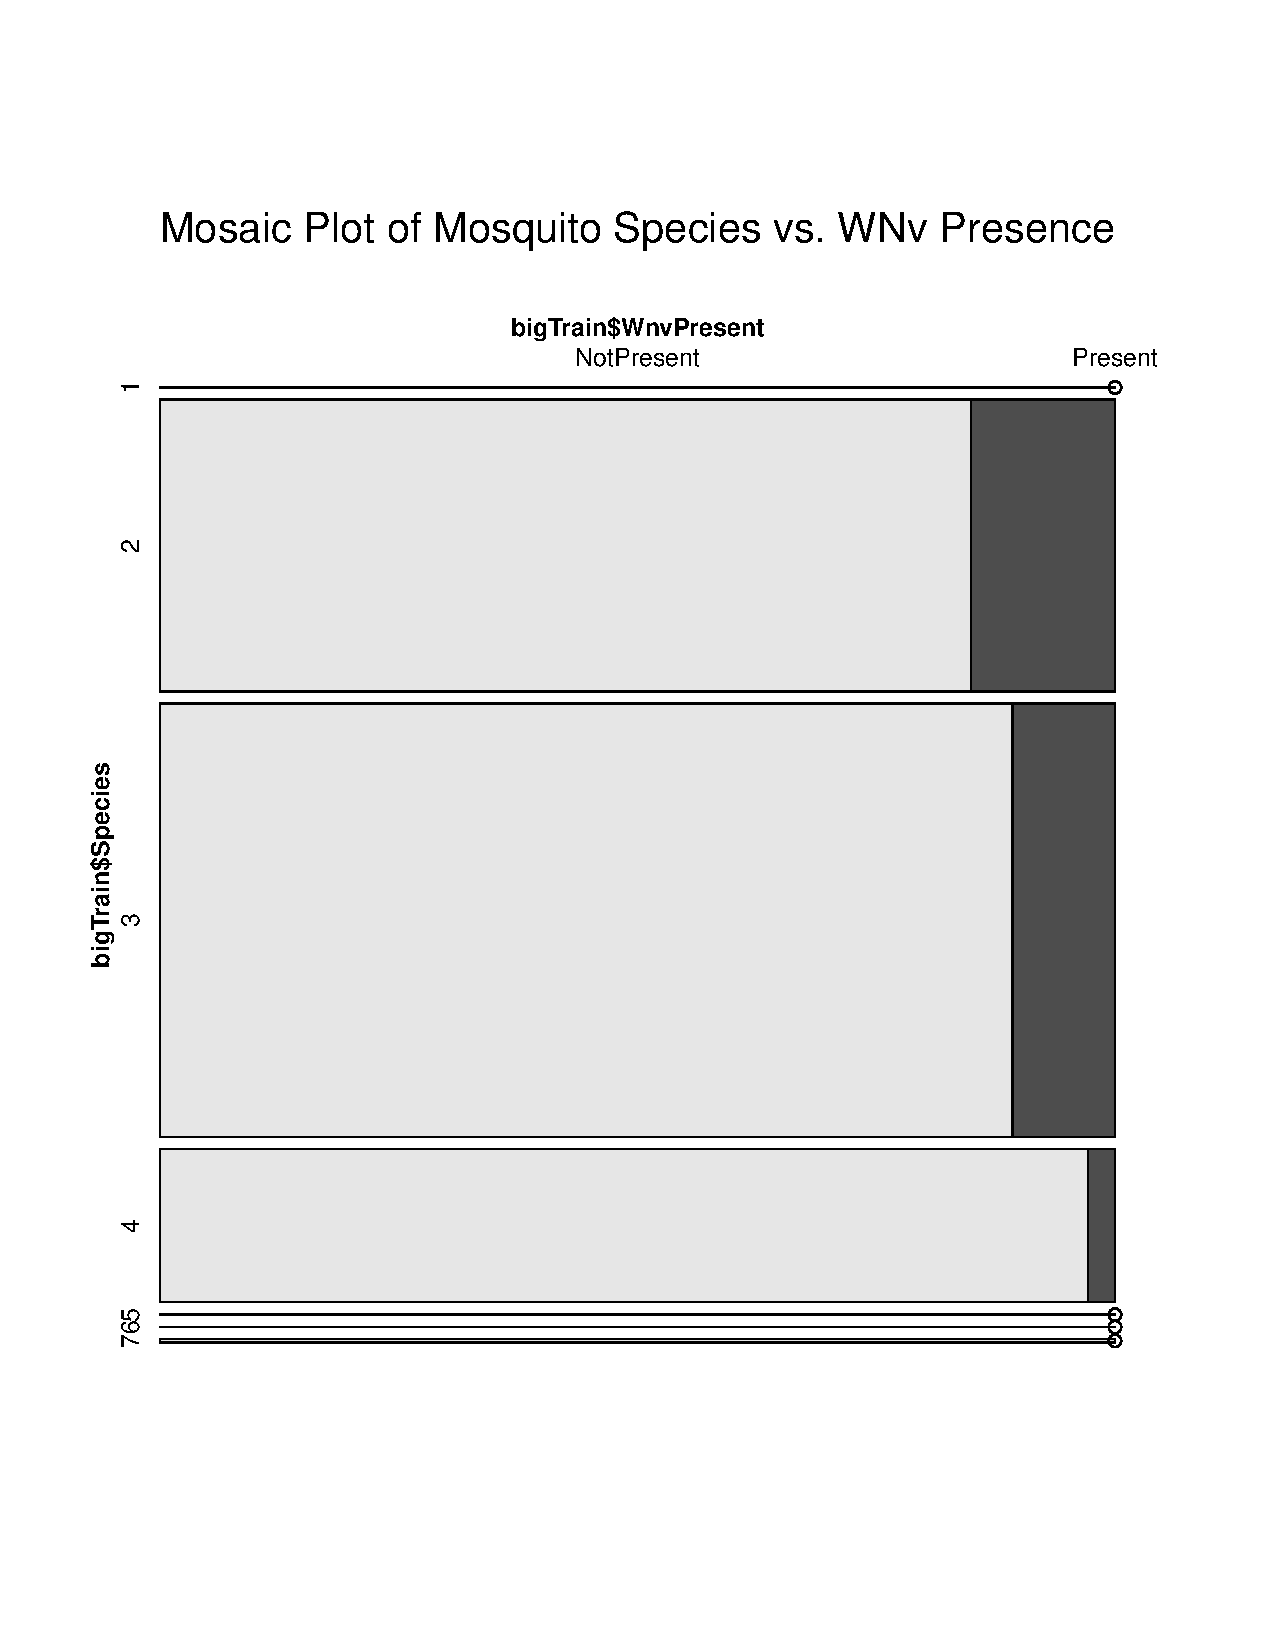
\includegraphics[height=7cm, width=10cm]{Mosaic_SpeciesVSWNv.pdf}
\end{figure}
\end{frame}

\begin{frame}
\frametitle{Location Effect}
\begin{figure}[H] \center
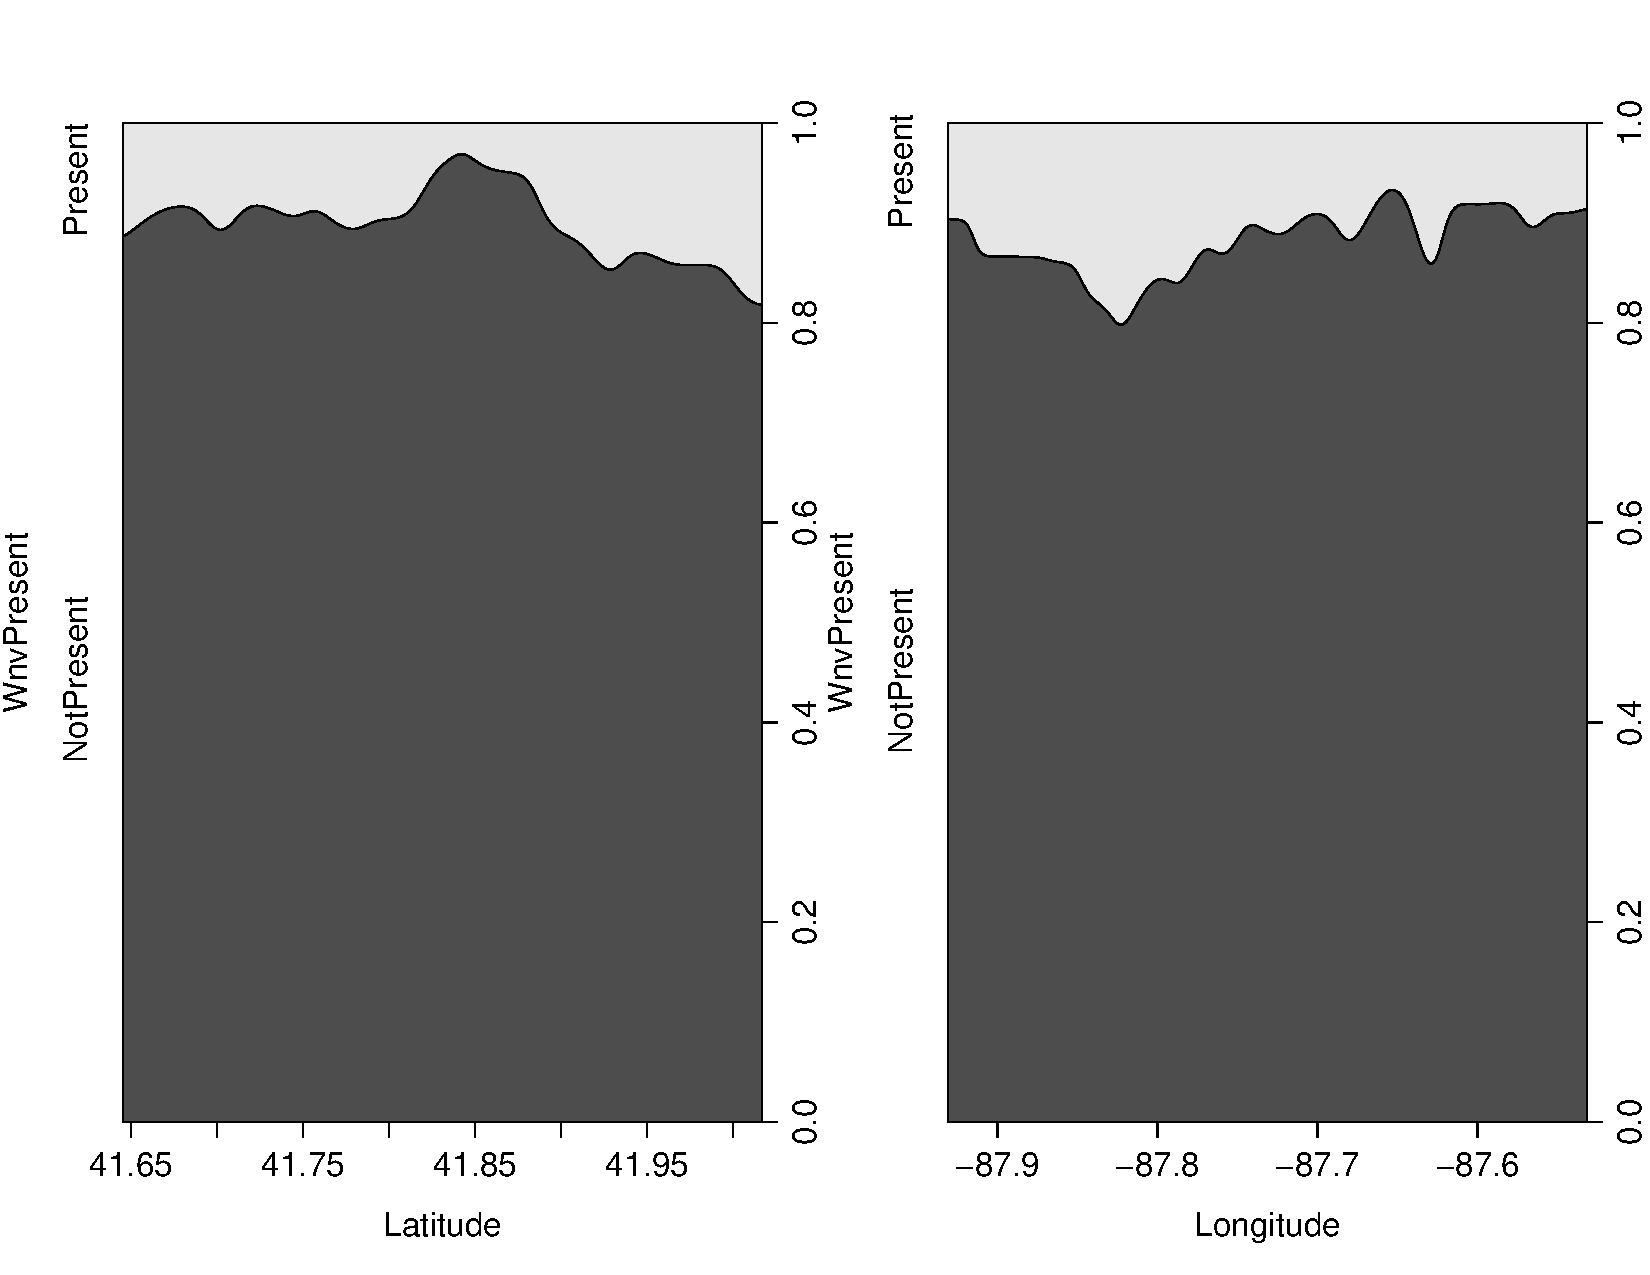
\includegraphics[scale=.30]{CD_LatLong.pdf}
\end{figure}
\end{frame}

\begin{frame}
\frametitle{Spray Effect}
\begin{itemize}
\item Compute Haversine distance for all spray and trap pairs.
${\scriptstyle d = 2 r \arcsin\left(\sqrt{\sin^2\left(\frac{\phi_2 - \phi_1}{2}\right) + \cos(\phi_1) \cos(\phi_2)\sin^2\left(\frac{\lambda_2 - \lambda_1}{2}\right)}\right)} $
\item For each trap, count how many sprays conducted within two miles and within two weeks of surveillance.
\end{itemize}
\begin{figure}[H] \center
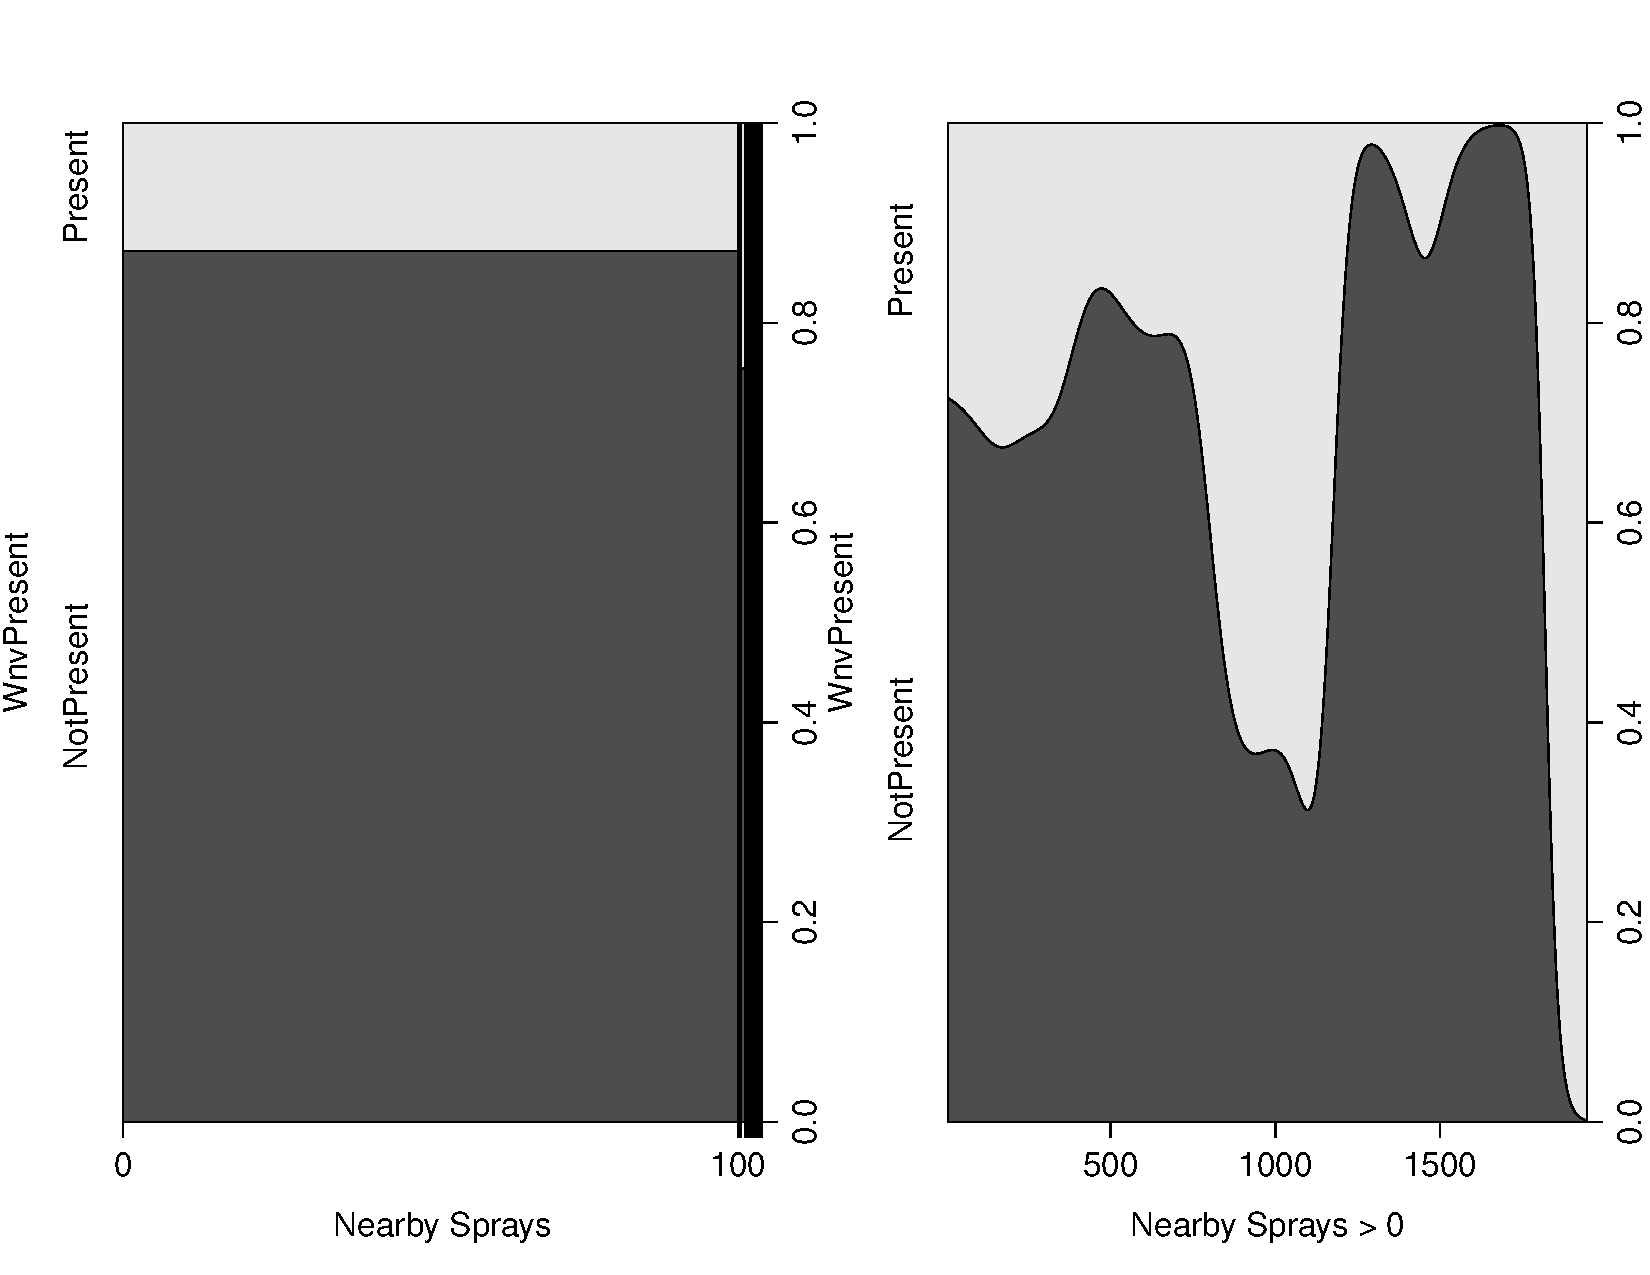
\includegraphics[height=5cm, width=10cm]{CD_NearbySpraysVSwnv.pdf}
\end{figure}
\end{frame}

\begin{frame}
\frametitle{Confirmatory Analysis}
\begin{scriptsize}
\begin{description}
\item[Full Logistic with weather, spray and trap predictors]\
\begin{itemize}
\item Poor model: Too complicated, strong collinearity, no significance
\item Ridge regression helps with collinearity, but not enough! Need to ``zero out'' terms
\end{itemize}
\item[ElasticNet]\
\begin{itemize}
\item Combination of Lasso and Ridge Regression, minimizes
$ \scriptstyle \frac{1}{N} \sum_{i=1}^{N} w_i l(y_i,\beta_0+\beta^T x_i) + \lambda\left[(1-\alpha)||\beta||_2^2/2 + \alpha ||\beta||_1\right] $
\item Like lasso, shrinks coefficients exactly to zero--produces simple models
\item Like ridge, doesn't just take one correlated predictor and leave the rest
\end{itemize}
\item[Generalized Additive Model (GAM)]\
\begin{itemize}
\item Allows non-linear terms
\item \emph{Far} better at modeling location effect.
\end{itemize}
\item[Generalized Linear Mixed Model (GLMM)]\
\begin{itemize}
\item Mosquitoes in the same trap are correlated! Account for it!
\end{itemize}
\end{description}
\end{scriptsize}
\end{frame}

\begin{frame}
\frametitle{Final Logistic Regression on Held-Out Data ($n=11,049$)}
\begin{center}
\begin{scriptsize}
\begin{tabular}{|c|cccc|c|} \hline
& Estimate & SE & $z$-value & $p$-value & VIF \\ \hline
(Intercept) & -470.5712 & 44.66 & -10.54 & $\ll 0.0001$ & - \\ 
isSpecies1247TRUE & -0.1289 & 0.06 & -2.05 & 0.0405 & 1.04\\ 
Longitude & -3.7336 & 0.60 & -6.21 & $\ll 0.0001$ & 4.08\\ 
Year2013 & 0.6037 & 0.11 & 5.70 & $\ll 0.0001$ & 1.89\\ 
Month7 & 2.3112 & 0.42 & 5.51 & $\ll 0.0001$ & 2.07\\ 
Month8 & 4.6864 & 0.42 & 11.28 & $\ll 0.0001$ & \\ 
Month9 & 4.4322 & 0.42 & 10.66 & $\ll 0.0001$ & \\ 
Tmax & 0.0712 & 0.01 & 8.34 & $\ll 0.0001$ & 3.97\\ 
HeatDegreeDay & 0.0781 & 0.02 & 3.19 & 0.0014 & 2.95\\ 
StationPressure & 3.9241 & 0.70 & 5.60 & $\ll 0.0001$ & 4.79\\ 
ResultSpeed & 0.0980 & 0.02 & 5.74 & $\ll 0.0001$ & 2.98\\ 
anyNearbySpraysTRUE & 0.5445 & 0.11 & 5.06 & $\ll 0.0001$ & 1.08\\ 
Latitude:Longitude & -0.0042 & 0.005 & -0.87 & 0.3859 & 4.04\\ \hline
\end{tabular}
\end{scriptsize}
\end{center}
\end{frame}

\section{Prediction}
\begin{frame}
\frametitle{Central Goal of Prediction}
\begin{center}
\textbf{Can we develop a tool that has high sensitivity to detect West Nile virus, while still maintaining specificity?}
\begin{scriptsize}
\begin{itemize}
\item On the whole data set (without Spray data)?
\item For 2011 and 2013 (with Spray and weather data)?
\item For 2011 and 2013 (with weather data only)?
\end{itemize}
\end{scriptsize}
\end{center}
\end{frame}

\begin{frame}
\frametitle{Tools}
\begin{description}
\item[GLM] Logistic regression, with no model selection.
\item[GLM-Net] GLM followed by optimally-tuned ElasticNets.
\item[RandomForest] CART-based ensemble, taking a random subset of data \emph{and} random subset of the \emph{predictors} for each tree. Trees then averaged to form classifier.
\item[Adaptive Boosting (AdaBoost)] Ensemble that builds really bad trees (``weak learners''), then tunes subsequent trees to perform better on the samples that the previous trees misclassified.
\item[Gradient Boosting Machines] Class of ensembles that includes AdaBoost. Allow for more general loss functions. Optimizes with gradient descent. Faster and more memory-efficient than AdaBoost.
\end{description}
\end{frame}

\begin{frame}
\frametitle{Models have fantastic accuracy, utterly useless}
\begin{itemize}
\item Unbalanced classes--can achieve great accuracy by always predicting to common class
\item Classification Accuracy and AUC are bad metrics for unbalanced responses.
\end{itemize}

\begin{center}
\begin{tabular}{|c|c|c|} \hline
\multicolumn{3}{|c|}{GLM-Net, SprayYears, All vars} \\ \hline
(In $\%$) & True $-$ & True $+$ \\ \hline 
Predict $-$ & $86.10$ & $12.50$ \\ \hline 
Predict $+$ & $0.5$ & $0.9$ \\ \hline 
\end{tabular} 
\end{center}
\end{frame}

\begin{frame}
\frametitle{Solutions}
\begin{itemize}
\item Need to balance high specificity (easy) with high sensitivity (very hard). Punish classifiers that ``cheat''.
\end{itemize}

\begin{description}
\item[Balanced Accuracy ($BA$)] \
\begin{itemize}
\item Mean of sensitivity and specificity
\item Weights desire to correctly classify WNv-negative and WNv-positive cases by their incidence.
\end{itemize}

\item[$F_1$ Score] \
\begin{itemize}
\item $F_1 = 2 \cdot \left( \mathrm{PPV} \cdot \mathrm{Sens} \right) / \left( \mathrm{PPV} + \mathrm{Sens}\right)$
\item Harmonic mean of Positive Predictive Value ($P(\text{WNv}+ | \text{Guess}+)$) and sensitivity
\item Tries to achieve high sensitivity, controlled by true WNv prevalence.
\end{itemize}
\end{description}
\end{frame}

\begin{frame}
\frametitle{Optimizing for $F_1$ and BA, instead...}

Confusion Matrices for $F_1$-based optimization (subset of table)
\begin{table}[H] \center \tiny
\begin{tabular}{|ll|rrrrr|} \hline
Method & Data & True Neg & False Neg & False Pos & True Pos & $F_1$ \\ \hline
GLM & AllYears, Weather & 89.10 & 10.50 & 0.10 & 0.30 & 0.05 \\ 
  ElasticNet & AllYears, Weather & 89.10 & 10.50 & 0.10 & 0.20 & 0.04 \\ 
  \bf{RandomForest} & \bf{AllYears, Weather} & 88.30 & 4.00 & 1.00 & 6.80 & \bf{0.73} \\ \hline

  GLM & SprayYears, Weather & 86.10 & 12.50 & 0.50 & 0.90 & 0.12 \\ 
  \bf{RandomForest} & \bf{SprayYears, Weather} & 85.20 & 3.40 & 1.40 & 10.00 & \bf{0.81} \\ 
  AdaBoost & SprayYears, Weather & 84.60 & 8.80 & 2.00 & 4.70 & 0.47 \\ \hline

  GLM & SprayWeather & 86.10 & 12.40 & 0.50 & 1.00 & 0.13 \\ 
  \bf{RandomForest} & \bf{SprayWeather} & 85.10 & 3.30 & 1.50 & 10.10 & \bf{0.81} \\ 
  AdaBoost & SprayWeather & 84.50 & 8.70 & 2.10 & 4.70 & 0.47 \\ \hline
\end{tabular}
\end{table}

Confusion Matrices for $BA$-based optimization (subset of table)
\begin{table}[H] \center \tiny
\begin{tabular}{|ll|rrrrr|} \hline
Method & Data & True Neg & False Neg & False Pos & True Pos & BA \\ \hline
GLM & AllYears, Weather & 89.10 & 10.50 & 0.10 & 0.30 & 0.51 \\ 
  ElasticNet & AllYears, Weather & 89.10 & 10.50 & 0.10 & 0.20 & 0.51 \\ 
  \bf{RandomForest} & \bf{AllYears, Weather} & 88.20 & 3.90 & 1.00 & 6.80 & \bf{0.81} \\ \hline

  GLM & SprayYears, Weather & 86.10 & 12.50 & 0.50 & 0.90 & 0.53 \\ 
  ElasticNet & SprayYears, Weather & 86.00 & 12.50 & 0.50 & 0.90 & 0.53 \\ 
  \bf{RandomForest} & \bf{SprayYears, Weather} & 85.00 & 3.20 & 1.50 & 10.20 & \bf{0.87} \\ 
  AdaBoost & SprayYears, Weather & 84.60 & 8.80 & 2.00 & 4.60 & 0.66 \\ \hline

  \bf{RandomForest} & \bf{SprayWeather} & 84.90 & 3.20 & 1.70 & 10.20 & \bf{0.87} \\ 
  GradientBoosting & SprayWeather & 84.50 & 5.00 & 2.10 & 8.40 & 0.80 \\ 
  AdaBoost & SprayWeather & 84.50 & 9.00 & 2.10 & 4.40 & 0.65 \\ \hline
\end{tabular}
\end{table}
\end{frame}

\section{Conclusion}
\begin{frame}
\frametitle{Concluding Remarks}
\begin{description}
\item[Regularization separates the wheat from the chaff]\
\begin{itemize}
\item Found very significant model
\item Parsimonious and intuitive to explain
\item Previous weather findings reinforced
\item Clear location effect
\end{itemize}
\item[Strong Spraying Effect, Interpretation Unclear]\
\begin{itemize}
\item Need better tools (spatiotemporal analysis)
\end{itemize}

\item[Accuracy is a bad choice with uneven frequencies]\
\begin{itemize}
\item GLMs are garbage at classification
\item $F_1$ and Balanced Accuracy give good sensitivity, decent specificity
\item ``Best'' classifier is dependent on desired properties (No Free Lunch)
\end{itemize}
\end{description}
\end{frame}

\begin{frame}
\frametitle{Parallel Programming Is \emph{Vital} to Predictive Modeling}
\begin{figure}[H]
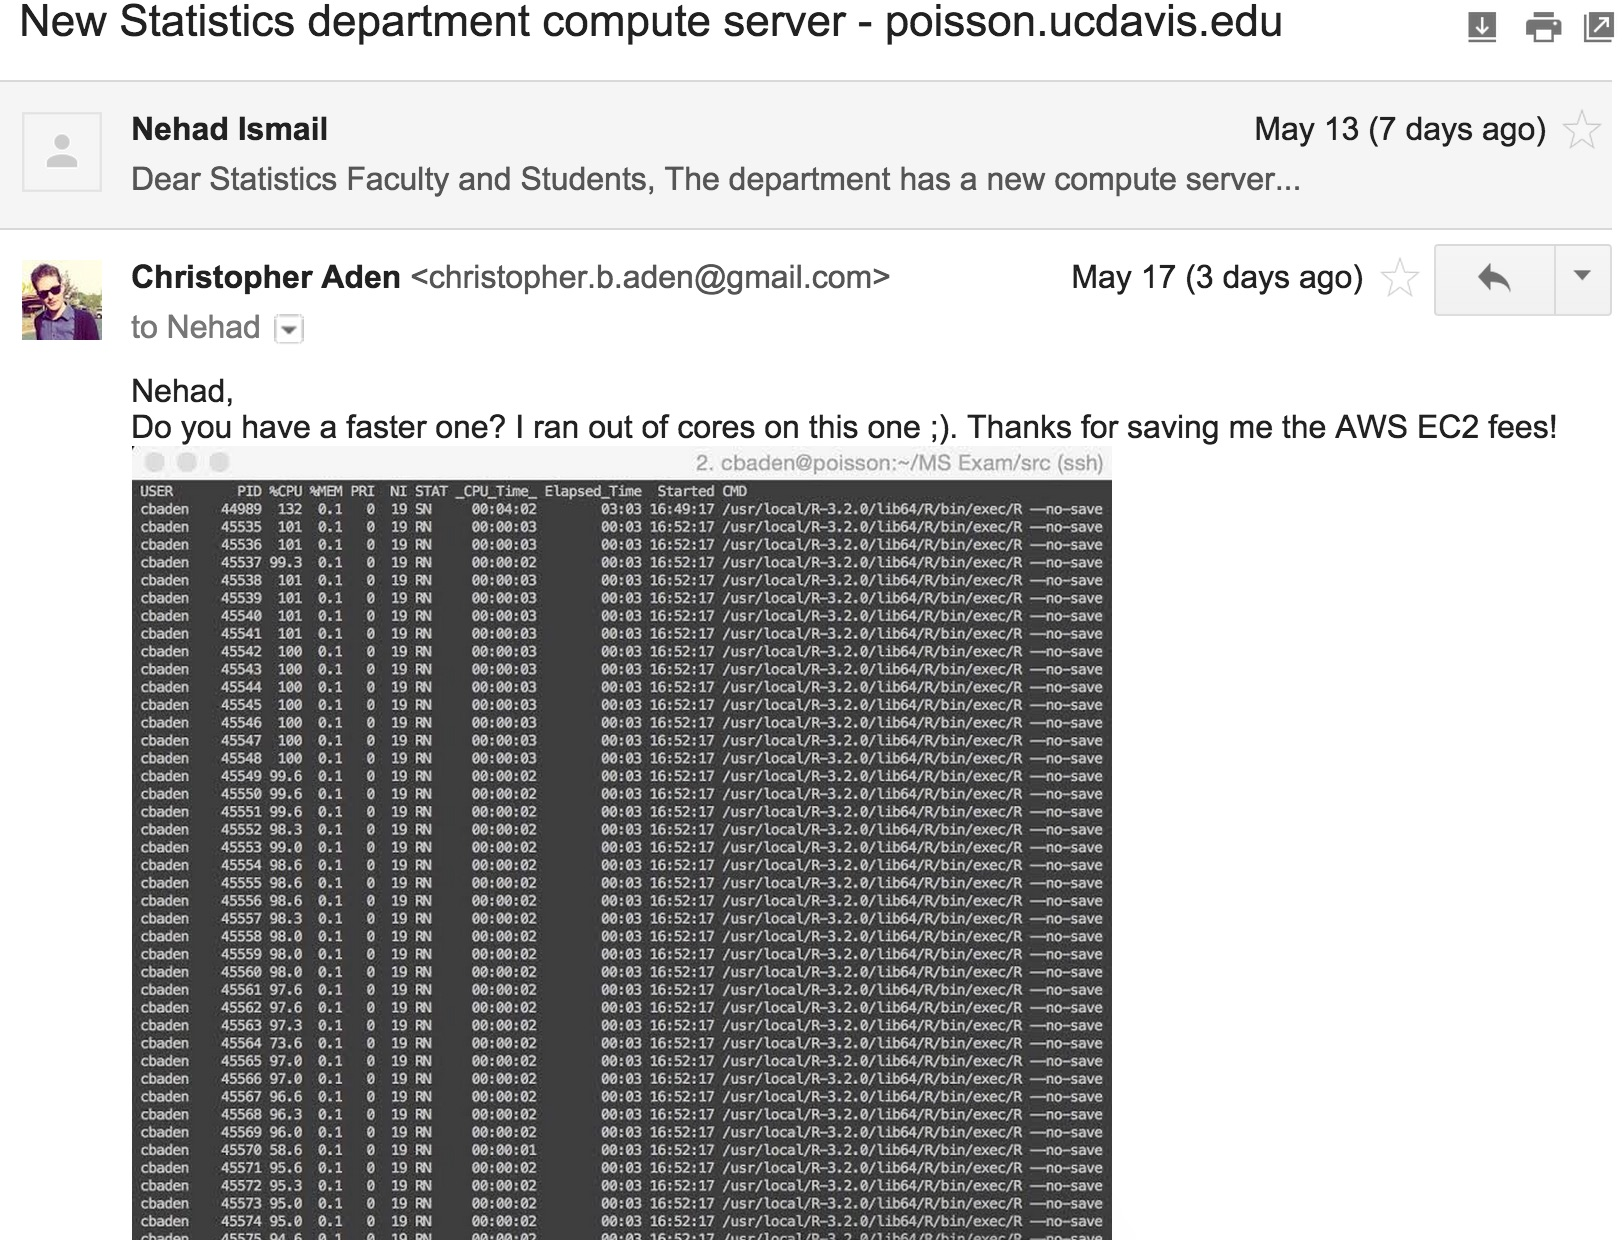
\includegraphics[width=10cm, height=10cm]{pp.jpg}
\end{figure}
\end{frame}
\end{document}